\section{Les pratiques du développeur}
\label{sec:pratiques}

\lstset{basicstyle=\ttfamily\tiny}

\subsection{Le nommage}
\label{subsec:pratiques-nommage}

\begin{frame}
    \frametitle{Choisir des noms qui ont du sens}

    \begin{columns}
        \begin{column}{0.5\textwidth}
            \lstinputlisting[
                language={[Sharp]C},
                label=lst:nommage-ko]
            {figures/pratiques/noms-ko.cs}
        \end{column}
        \pause
        \begin{column}{0.5\textwidth}
            \lstinputlisting[
                language={[Sharp]C},
                label=lst:nommage-ok]
            {figures/pratiques/noms-ok.cs}
        \end{column}
    \end{columns}
\end{frame}

%todo: détailler en exemples de code
\begin{frame}
    \frametitle{Une langue qui a du sens}

    \begin{itemize}
        \item Les noms des classes sont des noms ou des groupes nominaux ;
        \item Les noms des méthodes sont des verbes ou des groupes verbaux ;
        \item Choisir un mot par concepts ;
        \item Choisir des noms dans le domaine de la solution ;
        \item Choisir des noms dans le domaine du problème.
    \end{itemize}

    Ces points sont à rapprocher des notions
    de langage dédié (DSL) et de langage ubiquitaire.

\end{frame}

\subsection{Les fonctions}
\label{subsec:pratiques-fonctions}

\begin{frame}
    \frametitle{Des fonctions lisibles}

    \scalebox{.7}{
        \lstinputlisting[
            language={[Sharp]C},
            label=lst:fonction-ko]
        {figures/pratiques/fonction-ko.cs}
    }
\end{frame}

\begin{frame}
    \frametitle{Des fonctions lisibles}

    \lstinputlisting[
        language={[Sharp]C},
        label=lst:fonction-ok]
    {figures/pratiques/fonction-ok.cs}
\end{frame}

\begin{frame}
    \frametitle{Des fonctions lisibles}

    \lstinputlisting[
        language={[Sharp]C},
        label=lst:fonction-ok-best]
    {figures/pratiques/fonction-ok-best.cs}
\end{frame}

\begin{frame}
    \frametitle{Des fonctions lisibles}

    \begin{itemize}
        \item Faire court ;
        \item Faire une seule chose ;
        \item Un niveau d'abstraction par fonction.
    \end{itemize}
\end{frame}

%todo: détailler en exemples de code
\begin{frame}
    \frametitle{Arguments et retour d'une fonction}

    \begin{itemize}
        \item Idéalement, le nombre d’arguments d’une fonction devrait être égal à zéro ;
        \item Encapsuler dans des objets si plus de deux arguments ;
        \item Éviter les effets secondaires ;
        \item Éviter les arguments de sortie ;
        \item Séparer commandes et demandes ;
        \item Préférer les exceptions au retour de codes d’erreur ;
        \item Faire de la programmation structurée.
    \end{itemize}
\end{frame}

\subsection{Les commentaires}
\label{subsec:pratiques-commentaires}

\begin{frame}
    \frametitle{Les commentaires ne compensent pas du mauvais code}

    \begin{columns}
        \begin{column}{0.5\textwidth}
            \lstinputlisting[
                language={[Sharp]C},
                label=lst:comment-ko]
            {figures/pratiques/comment-ko.cs}
        \end{column}
        \pause
        \begin{column}{0.5\textwidth}
            \lstinputlisting[
                language={[Sharp]C},
                label=lst:comment-ok]
            {figures/pratiques/comment-ok.cs}
        \end{column}
    \end{columns}
\end{frame}

\begin{frame}
    \frametitle{Des commentaires informatifs}

    \lstinputlisting[
        language={[Sharp]C},
        label=lst:comment-inform]
    {figures/pratiques/comment-inform.cs}
\end{frame}

\begin{frame}
    \frametitle{Expliquer les intentions}

    \lstinputlisting[
        language={[Sharp]C},
        label=lst:comment-intention]
    {figures/pratiques/comment-intention.cs}
\end{frame}

\begin{frame}
    \frametitle{Avertir des conséquences}

    \lstinputlisting[
        language={[Sharp]C},
        label=lst:comment-avertir]
    {figures/pratiques/comment-avertir.cs}
\end{frame}

\begin{frame}
    \frametitle{Les mauvais commentaires}

    \lstinputlisting[
        language={[Sharp]C},
        label=lst:comment-mauvais]
    {figures/pratiques/comment-mauvais.cs}
\end{frame}

\subsection{Les structures de données}
\label{subsec:pratiques-types}

\begin{frame}
    \frametitle{Abstraction de données}

    Si nous voulons que nos variables soient privées, c’est pour une bonne raison :
    nous voulons que personne d’autre en dépende.
    Nous voulons garder la liberté de modifier leur type ou leur implémentation
    sur un coup de tête ou une envie soudaine.

    \bigskip
    Dans ce cas, pourquoi tant de programmeurs ajoutent automatiquement
    des accesseurs (méthodes get et set) à leurs objets,
    exposant ainsi leurs variables privées comme si elles étaient publiques ?
\end{frame}

\begin{frame}
    \frametitle{Abstraction de données}

    \begin{columns}
        \begin{column}{0.5\textwidth}
            \lstinputlisting[
                language={[Sharp]C},
                label=lst:data-concrete]
            {figures/pratiques/data-concrete.cs}
        \end{column}
        \pause
        \begin{column}{0.5\textwidth}
            \lstinputlisting[
                language={[Sharp]C},
                label=lst:data-abstract]
            {figures/pratiques/data-abstract.cs}
        \end{column}
    \end{columns}
\end{frame}

\begin{frame}
    \frametitle{Loi de Déméter}

    Un module ne doit pas connaître les détails internes des objets qu’il manipule.

    \bigskip
    Plus précisément,
    une méthode f d’une classe C ne doit appeler que les méthodes des éléments suivants :
    \begin{itemize}
        \item C ;
        \item un objet créé par f ;
        \item un objet passé en argument à f ;
        \item un objet contenu dans une variable d’instance de C.
    \end{itemize}
\end{frame}

\begin{frame}
    \frametitle{Les objets de transfert de données (DTO)}

    \lstinputlisting[
        language={[Sharp]C},
        label=lst:data-transfer-object]
    {figures/pratiques/data-transfer-object.cs}
\end{frame}

\begin{frame}
    \frametitle{Les objets de transfert de données (DTO)}

    \begin{itemize}
        \item La forme la plus pure d’une structure de données est
        une classe avec des variables publiques et aucune fonction.
        Les DTO sont des structures très utiles, en particulier
        pour les communications avec les bases de données ou les clients.
        \item Les enregistrements actifs (Active Record) sont des formes particulières de DTO. Il
        s’agit de structures de données avec des variables publiques,
        mais qui offrent généralement des fonctions de navigation telles que save et find.
    \end{itemize}
\end{frame}

\subsection{La gestion des erreurs}
\label{subsec:pratiques-erreurs}

%todo: ajouter d'autres exemples de gestion d'erreurs

\begin{frame}
    \frametitle{Les null}

    \lstinputlisting[
        language={[Sharp]C},
        label=lst:error-null]
    {figures/pratiques/error-null.cs}
\end{frame}

\subsection{Les classes}
\label{subsec:pratiques-classes}

\begin{frame}
    \frametitle{SOLID}

    \begin{columns}
        \begin{column}{0.5\textwidth}
            \begin{itemize}
                \item Principe de responsabilité unique
                \item Principe ouvert/fermé
                \item Principe de substitution de Liskov
                \item Principe de ségrégation des interfaces
                \item Principe d'inversion des dépendances
            \end{itemize}
        \end{column}
        \begin{column}{0.5\textwidth}
            \begin{itemize}
                \item Single Responsibility Principle
                \item Open/closed principle
                \item Liskov substitution principle
                \item Interface segregation principle
                \item Dependency inversion principle
            \end{itemize}
        \end{column}
    \end{columns}
\end{frame}

\begin{frame}
    \frametitle{Principe de responsabilité unique}

    \begin{columns}
        \begin{column}{0.5\textwidth}
            \lstinputlisting[
                language={[Sharp]C},
                label=lst:srp-ko]
            {figures/pratiques/srp-ko.cs}
        \end{column}
        \pause
        \begin{column}{0.5\textwidth}
            \lstinputlisting[
                language={[Sharp]C},
                label=lst:srp-ok]
            {figures/pratiques/srp-ok.cs}
        \end{column}
    \end{columns}
\end{frame}

\begin{frame}
    \frametitle{Principe de responsabilité unique}

    Une classe doit avoir une et une seule raison de changer !

    \begin{itemize}
        \item La classe est plus facile à comprendre ;
        \item La classe est plus facile à maintenir ;
        \item La classe est plus réutilisable.
    \end{itemize}

    \bigskip
    Le SRP équivaut à peu près à avoir une \textbf{« cohésion élevée »}.
    On dit qu’une classe a une forte cohésion si ses comportements sont fortement liés et fortement concentrés.
    Le SRP stipule qu’une classe doit être cohérente au point d’avoir une seule responsabilité,
    où une responsabilité est définie comme \textbf{« une raison de changement »}.

\end{frame}

\begin{frame}
    \frametitle{Principe ouvert/fermé}

    \begin{columns}
        \begin{column}{0.5\textwidth}
            \lstinputlisting[
                language={[Sharp]C},
                label=lst:ocp-ko]
            {figures/pratiques/ocp-ko.cs}
        \end{column}
        \pause
        \begin{column}{0.5\textwidth}
            \lstinputlisting[
                language={[Sharp]C},
                label=lst:ocp-ok]
            {figures/pratiques/ocp-ok.cs}
        \end{column}
    \end{columns}
\end{frame}


\begin{frame}
    \frametitle{Principe ouvert/fermé}

    Vous devriez pouvoir étendre le comportement d'une classe, sans le modifier.\\
    Une classe doit être ouverte à l’extension, mais fermée à la modification.

    \begin{itemize}
        \item La classe devient robuste, flexible et réutilisable ;
        \item Moins de modification implique moins de bogue.
    \end{itemize}

\end{frame}

\begin{frame}
    \frametitle{Principe de substitution de Liskov}

    \begin{columns}
        \begin{column}{0.5\textwidth}
            \lstinputlisting[
                language={[Sharp]C},
                label=lst:lsp-ko]
            {figures/pratiques/lsp-ko.cs}
        \end{column}
        \pause
        \begin{column}{0.5\textwidth}
            \lstinputlisting[
                language={[Sharp]C},
                label=lst:lsp-ok]
            {figures/pratiques/lsp-ok.cs}
        \end{column}
    \end{columns}
\end{frame}

\begin{frame}
    \frametitle{Principe de substitution de Liskov}

    Les fonctions qui utilisent une classe de base doivent
    pouvoir utiliser des objets de classes dérivées sans le savoir.

    Lorsque les sous-classes n'adhèrent pas correctement à l'interface de la classe de base,
    il faut parcourir le code existant et tenir compte des cas particuliers impliquant les sous-classes délinquantes.
    Il s’agit d’une violation flagrante du principe ouvert/fermé.

    \bigskip
    Lors de l’apprentissage de la programmation orientée objet,
    l’héritage est généralement décrit comme une relation « est un »,
    mais elle entraîne \textbf{parfois une mauvaise utilisation de l'héritage}.

\end{frame}

\begin{frame}
    \frametitle{Principe de ségrégation des interfaces}

    \begin{columns}
        \begin{column}{0.5\textwidth}
            \lstinputlisting[
                language={[Sharp]C},
                label=lst:isp-ko]
            {figures/pratiques/isp-ko.cs}
        \end{column}
        \pause
        \begin{column}{0.5\textwidth}
            \lstinputlisting[
                language={[Sharp]C},
                label=lst:isp-ok]
            {figures/pratiques/isp-ok.cs}
        \end{column}
    \end{columns}
\end{frame}

\begin{frame}
    \frametitle{Principe de ségrégation des interfaces}

    Les clients ne devraient pas être obligés de dépendre d’interfaces qu’ils n’utilisent pas.

    Ce principe permet d'éviter le couplage involontaire entre classes.
\end{frame}

\begin{frame}
    \frametitle{ISP, OCP, and DIP… OMG WTF BBQ?}

    L'exemple précédent ne viole pas simplement la ségrégation des interfaces (ISP),
    il viole également inversion de dépendance (DIP) et le principe d'ouverture/fermeture (OCP).
    C’est assez courant, donc si vous adhérez correctement au DIP et à l’OCP,
    vous ne rencontrerez pas de nombreuses violations de l'ISP.
    Cela dit, c'est un autre moyen pratique d'évaluer la conception de votre classe.

    \bigskip
    \textbf{``Ai-je besoin de toutes les méthodes de cette interface que j'utilise ?''}

    Si la réponse est non, vous souhaiterez peut-être utiliser une interface différente
    et appliquer certains des autres principes SOLID.
\end{frame}

\begin{frame}
    \frametitle{Principe d'inversion des dépendances}

    \begin{columns}
        \begin{column}{0.5\textwidth}
            \lstinputlisting[
                language={[Sharp]C},
                label=lst:dip-ko]
            {figures/pratiques/dip-ko.cs}
        \end{column}
        \pause
        \begin{column}{0.5\textwidth}
            \lstinputlisting[
                language={[Sharp]C},
                label=lst:dip-ok]
            {figures/pratiques/dip-ok.cs}
        \end{column}
    \end{columns}
\end{frame}

\begin{frame}
    \frametitle{Principe d'inversion des dépendances}

    Les modules de haut niveau ne doivent pas dépendre de modules de bas niveau.
    Les deux devraient dépendre d’abstractions.

    Ce principe permet de réduire le couplage entre composants.

    \bigskip
    Le principe d'inversion de dépendance est essentiellement un moyen d'ajouter des fiches et des prises à votre code.
    Il vous permet de créer des modules de haut niveau indépendants des modules de bas niveau.
    Les modules de bas niveau peuvent être créés ultérieurement et sont facilement remplaçables.
\end{frame}

\begin{frame}
    \frametitle{SOLID en une seule diapositive}

    \centering
    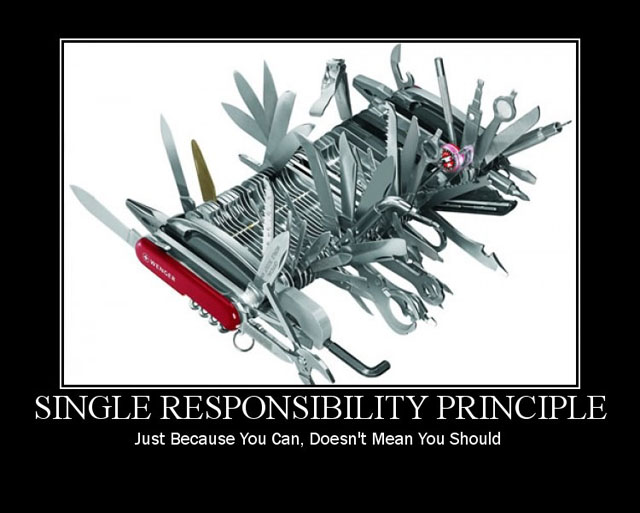
\includegraphics[height=100px]{figures/pratiques/srp}
    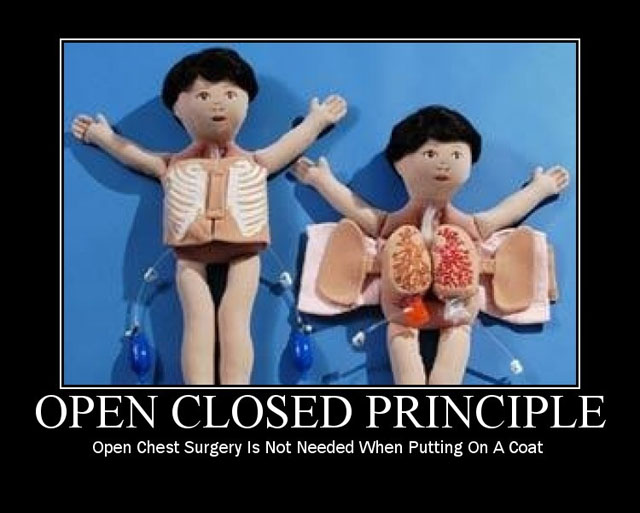
\includegraphics[height=100px]{figures/pratiques/ocp}
    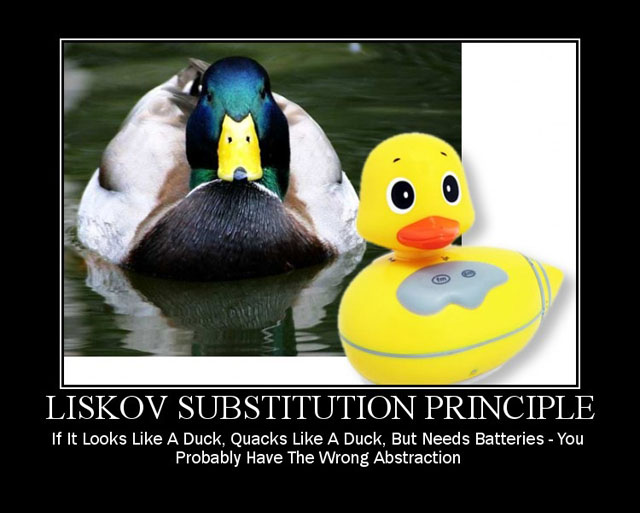
\includegraphics[height=100px]{figures/pratiques/lsp}

    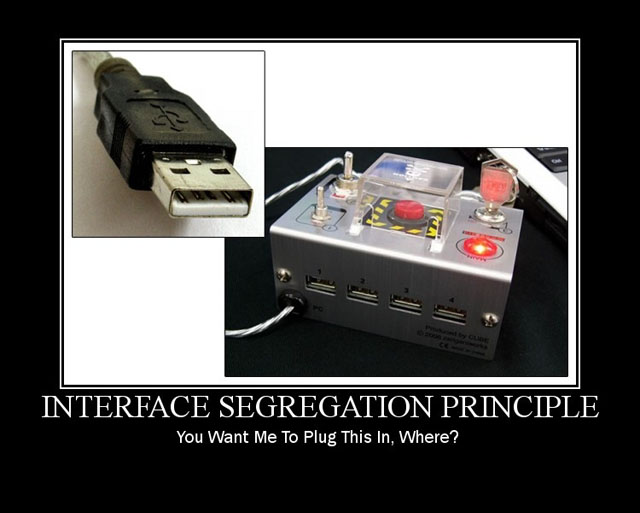
\includegraphics[height=100px]{figures/pratiques/isp}
    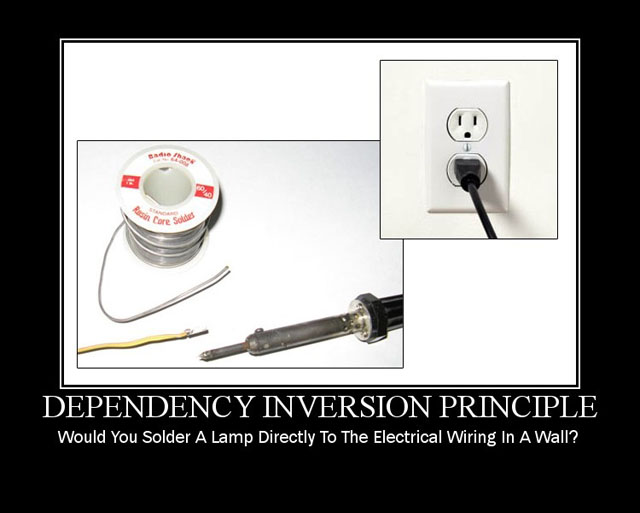
\includegraphics[height=100px]{figures/pratiques/dip}

\end{frame}

%todo: https://www.cynicalturtle.net/kame/post/2023/04/09/Affordance-trompeuse-les-bonnes-pratiques
%todo: lien clean code

\begin{frame}
    \centering
    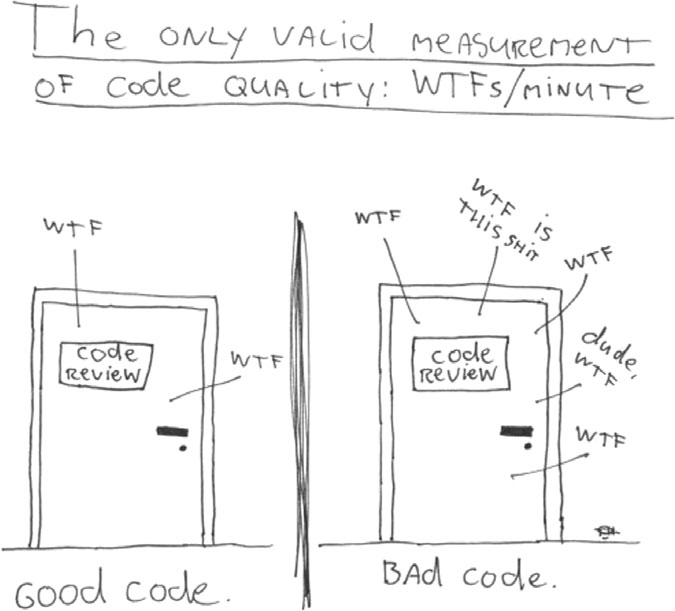
\includegraphics[height=0.5\linewidth]{figures/pratiques/wtf}
\end{frame}
